\documentclass[aspectratio=169,xcolor={dvipsnames}]{beamer}

% XeLaTeX packages
\usepackage{fontspec}
\usepackage{xcolor}
\usepackage{tikz}
\usetikzlibrary{positioning}
\usepackage{booktabs}
\usepackage{amsmath}
\usepackage{amsthm}
\usepackage{caption}
\usepackage{graphicx}
\usepackage{listings}
\usepackage{biblatex}

% Bibliography
\addbibresource{references_new.bib}

% Modern theme configuration
\usetheme{Boadilla}
\usecolortheme{default}

% Define complementary palette based on VU Blue
\definecolor{VUBlue}{HTML}{0057B7}
\definecolor{Endeavour}{HTML}{0754AA}
\definecolor{AbsoluteZero}{HTML}{055AB9}
\definecolor{ScienceBlue}{HTML}{0360C8}
\definecolor{RustyNail}{HTML}{8E4F09}
\definecolor{RichGold}{HTML}{9C5608}
\definecolor{LightGray}{HTML}{E8E9EA}
\definecolor{Charcoal}{HTML}{222831}

% Set theme colors
\setbeamercolor{frametitle}{bg=VUBlue, fg=white}
\setbeamercolor{title}{fg=VUBlue}
\setbeamercolor{structure}{fg=ScienceBlue}
\setbeamercolor{alerted text}{fg=RustyNail}
\setbeamercolor{block title}{bg=AbsoluteZero, fg=white}
\setbeamercolor{block body}{bg=LightGray, fg=Charcoal}
\setbeamercolor{alertblock title}{bg=RustyNail, fg=white}
\setbeamercolor{alertblock body}{bg=LightGray, fg=Charcoal}

% Font settings
\setmainfont{Liberation Sans}
\setsansfont{Liberation Sans}
\setmonofont{Liberation Mono}[Scale=0.9]

% Custom commands
\newcommand{\highlight}[1]{\textcolor{RustyNail}{\textbf{#1}}}
\newcommand{\code}[1]{\texttt{\small #1}}
\newcommand{\phase}[1]{\textcolor{ScienceBlue}{\textbf{Phase #1}}}

% Configure listings
\lstset{
  basicstyle=\ttfamily\footnotesize,
  backgroundcolor=\color{LightGray},
  frame=single,
  breaklines=true
}

% Title page info
\title{Privacy-Preserving Synthetic Trajectory Generation}
\subtitle{An Integrated DiffTraj-LM-TAD Framework for Taxi Route Anomaly Detection}
\author{Mateusz Kędzia}
\institute{MSc AI \\ VUA / BJUT}
\date{Thesis Methodology Presentation -- July 2025}

% Custom title page
\defbeamertemplate*{title page}{customized}[1][]
{%
  \vbox{}
  \vfill
  \begingroup
    \centering
    \begin{beamercolorbox}[sep=8pt,center,#1]{title}
      \usebeamerfont{title}\inserttitle\par%
      \ifx\insertsubtitle\@empty%
      \else%
        \vskip0.25em%
        {\usebeamerfont{subtitle}\usebeamercolor[fg]{subtitle}\insertsubtitle\par}%
      \fi%     
    \end{beamercolorbox}%
    \vskip1em\par
    \begin{beamercolorbox}[sep=8pt,center,#1]{author}
      \usebeamerfont{author}\insertauthor
    \end{beamercolorbox}
    \begin{beamercolorbox}[sep=8pt,center,#1]{institute}
      \usebeamerfont{institute}\insertinstitute
    \end{beamercolorbox}
    \begin{beamercolorbox}[sep=8pt,center,#1]{date}
      \usebeamerfont{date}\insertdate
    \end{beamercolorbox}\vskip0.5em
  \endgroup
  \vfill
}

\begin{document}

% --- Title Slide ---
\begin{frame}[plain]
  \vspace{1.5cm}
  \centering
  {\usebeamerfont{title}\color{VUBlue}\Huge\textbf{Privacy-Preserving Synthetic Trajectory Generation}}
  
  \vspace{0.5em}
  {\usebeamerfont{subtitle}\color{RichGold}\Large An Integrated DiffTraj-LM-TAD Framework}
  
  \vspace{1.5em}
  {\usebeamerfont{author}\large Mateusz Kędzia}
  
  \vspace{0.5em}
  {\usebeamerfont{institute}\normalsize MSc Artificial Intelligence \\ Vrije Universiteit Amsterdam}
  
  \vspace{1em}
  {\usebeamerfont{date}\small Thesis Progress Presentation -- July 2025}
\end{frame}

% --- Problem & Solution ---
\begin{frame}{The Challenge}
  \begin{alertblock}{Privacy vs. Utility Paradox}
    \centering
    \Large Traditional privacy methods degrade spatio-temporal patterns needed for anomaly detection \cite{buchholzSystematisationKnowledgeTrajectory2024}
  \end{alertblock}
  
  \vspace{1em}
  \begin{block}{Solution: A Self-Sufficient Data Generation Cycle}
    \centering
    Resolve the paradox by creating labeled anomaly data from a private, synthetic source.
    \vspace{1em}
    
    
\begin{tikzpicture}[node distance=0.2cm, every node/.style={font=\large}]
      \node (private) {\textbf{\color{ScienceBlue}Private Data}};
      \node[right=of private] (arrow1) {$\boldsymbol{\rightarrow}$};
      \node[right=of arrow1] (anomalous) {\textbf{\color{RustyNail}Mined Anomalies}};
      \node[right=of anomalous] (arrow2) {$\boldsymbol{\rightarrow}$};
      \node[right=of arrow2] (utility) {\textbf{\color{AbsoluteZero}High-Utility Model}};
    \end{tikzpicture}
  \end{block}
\end{frame}

% --- Core Process Overview ---
\begin{frame}{3-Phase Bootstrap Framework}
  \begin{center}
    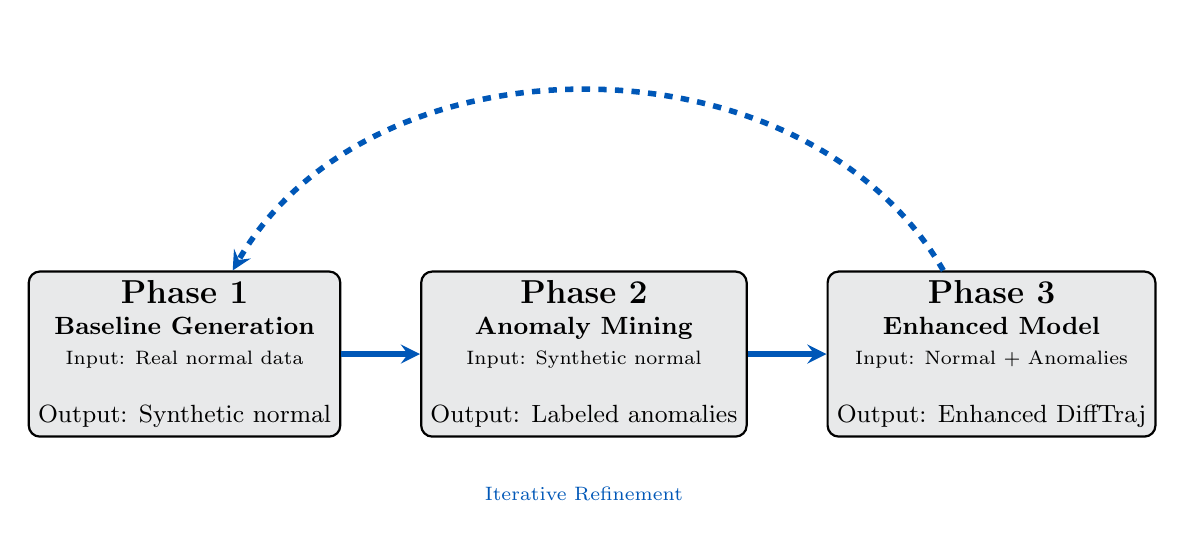
\begin{tikzpicture}[
      node distance=1.0cm,
      every node/.style={align=center, font=\small},
      box/.style={draw, fill=LightGray, rounded corners, minimum width=2.8cm, minimum height=2cm, thick},
      arrow/.style={thick, VUBlue, ->, >=stealth, line width=2pt}
    ]
      % Phase boxes
      \node[box] (phase1) {\textbf{\large Phase 1}\\\textbf{Baseline Generation}\\\vspace{0.3cm}\scriptsize Input: Real normal data\\Output: Synthetic normal};
      \node[box, right=of phase1] (phase2) {\textbf{\large Phase 2}\\\textbf{Anomaly Mining}\\\vspace{0.3cm}\scriptsize Input: Synthetic normal\\Output: Labeled anomalies};
      \node[box, right=of phase2] (phase3) {\textbf{\large Phase 3}\\\textbf{Enhanced Model}\\\vspace{0.3cm}\scriptsize Input: Normal + Anomalies\\Output: Enhanced DiffTraj};
      % Arrows
      \draw[arrow] (phase1) -- (phase2);
      \draw[arrow] (phase2) -- (phase3);
      % Feedback loop
      \draw[arrow, dashed] (phase3) to[bend right=60] (phase1);
      \node[below=0.5cm of phase2, font=\scriptsize\color{VUBlue}] {Iterative Refinement};
    \end{tikzpicture}
  \end{center}
\end{frame}

% --- DiffTraj Slide ---
\begin{frame}{Core Component 1: DiffTraj}
    \begin{block}{Generative Trajectory Synthesis \cite{zhuDiffTrajGeneratingGPS2023}}
        \small
        DiffTraj uses a diffusion model, a type of generative model, to create realistic, privacy-preserving GPS trajectories.
        \vspace{1em}
        \begin{itemize}
            \item \textbf{Forward Process:} Gradually adds Gaussian noise to real trajectories over many steps, eventually turning them into pure noise.
            \item \textbf{Reverse Process:} A neural network (Traj-UNet) learns to reverse this process. It takes random noise and, step-by-step, removes the noise to generate a clean, synthetic trajectory.
        \end{itemize}
    \end{block}
    
    \vspace{0.5em}
    \begin{alertblock}{Key Idea: Privacy from Noise}
        \centering
        \small
        Since synthetic trajectories are generated from random noise, they are not a copy or perturbation of any single real trajectory. This provides strong privacy guarantees by design.
    \end{alertblock}
\end{frame}

% --- LM-TAD Slide ---
\begin{frame}{Core Component 2: LM-TAD}
    \begin{block}{Anomaly Detection as a Language Problem \cite{mbuyaTrajectoryAnomalyDetection2024}}
        \small
        LM-TAD treats trajectories like sentences. Just as a language model learns grammar, LM-TAD learns the "grammar" of normal movement.
        \vspace{1em}
        \begin{itemize}
            \item \textbf{Tokenization:} A trajectory (a sequence of GPS points) is converted into a sequence of discrete tokens, similar to words in a sentence.
            \item \textbf{Perplexity Scoring:} The model calculates the \textit{perplexity} for a new trajectory. A high perplexity score means the sequence is "surprising" or unlikely, flagging it as a potential anomaly.
        \end{itemize}
    \end{block}

    \vspace{0.5em}
    \begin{alertblock}{Key Idea: Anomalies are "Ungrammatical" Trajectories}
        \centering
        \small
        Anomalies are detected because they violate the learned probabilistic rules of normal movement, just like an ungrammatical sentence violates the rules of a language.
    \end{alertblock}
\end{frame}

% --- Phase 1 Detail ---
\begin{frame}{Phase 1: Baseline Generation}
  \begin{center}
    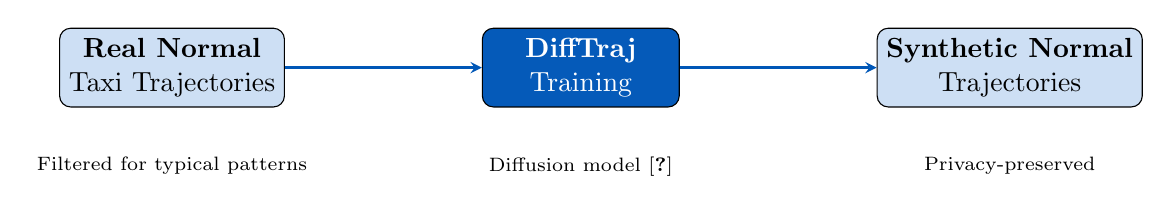
\begin{tikzpicture}[
      node distance=2.5cm,
      every node/.style={align=center},
      data/.style={draw, fill=ScienceBlue!20, rounded corners, minimum width=2cm, minimum height=1cm},
      process/.style={draw, fill=AbsoluteZero, text=white, rounded corners, minimum width=2.5cm, minimum height=1cm},
      arrow/.style={thick, VUBlue, ->, >=stealth}
    ]
      \node[data] (input) {\textbf{Real Normal}\\Taxi Trajectories};
      \node[process, right=of input] (difftraj) {\textbf{DiffTraj}\\Training};
      \node[data, right=of difftraj] (output) {\textbf{Synthetic Normal}\\Trajectories};
      \draw[arrow] (input) -- (difftraj);
      \draw[arrow] (difftraj) -- (output);
      % Labels
      \node[below=0.5cm of input, font=\scriptsize] {Filtered for typical patterns};
      \node[below=0.5cm of difftraj, font=\scriptsize] {Diffusion model \cite{zhuDiffTrajGeneratingGPS2023}};
      \node[below=0.5cm of output, font=\scriptsize] {Privacy-preserved};
    \end{tikzpicture}
  \end{center}
  \vspace{1em}
  \begin{block}{Key Innovation: Privacy by Sampling}
    Synthetic trajectories are generated by sampling from noise, decoupling outputs from any individual real trajectory.
  \end{block}
\end{frame}

% --- Phase 2 Detail ---
\begin{frame}{Phase 2: Anomaly Mining}
  \begin{center}
    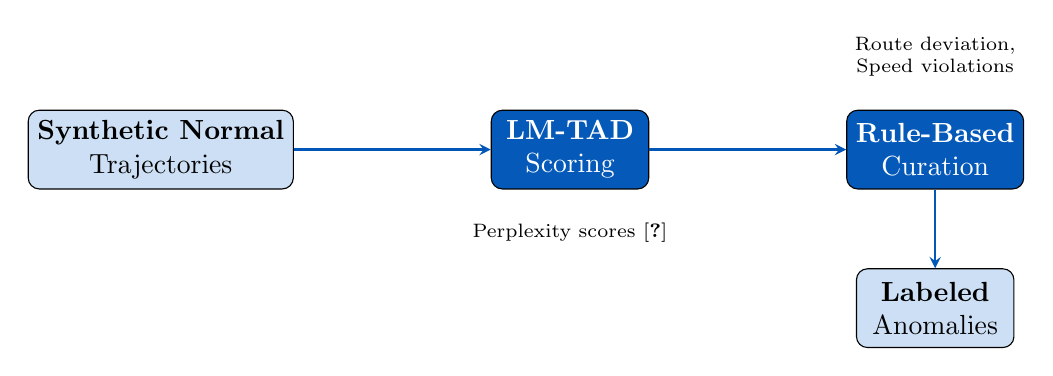
\begin{tikzpicture}[
      node distance=2.5cm,
      every node/.style={align=center},
      data/.style={draw, fill=ScienceBlue!20, rounded corners, minimum width=2cm, minimum height=1cm},
      process/.style={draw, fill=AbsoluteZero, text=white, rounded corners, minimum width=2cm, minimum height=1cm},
      arrow/.style={thick, VUBlue, ->, >=stealth}
    ]
      
      \node[data] (input) {\textbf{Synthetic Normal}\\Trajectories};
      \node[process, right=of input] (lmtad) {\textbf{LM-TAD}\\Scoring};
      \node[process, right=of lmtad] (rules) {\textbf{Rule-Based}\\Curation};
      \node[data, below=1cm of rules] (output) {\textbf{Labeled}\\Anomalies};
      
      \draw[arrow] (input) -- (lmtad);
      \draw[arrow] (lmtad) -- (rules);
      \draw[arrow] (rules) -- (output);
      
      % Labels
      \node[below=0.3cm of lmtad, font=\scriptsize] {Perplexity scores \cite{mbuyaTrajectoryAnomalyDetection2024}};
      \node[above=0.3cm of rules, font=\scriptsize] {Route deviation,\\Speed violations};
      
    \end{tikzpicture}
  \end{center}
  
  \vspace{1em}
  \begin{block}{Self-supervised Detection}
    LM-TAD treats trajectories as token sequences, identifying anomalies through language modeling perplexity
  \end{block}
\end{frame}

% --- Phase 3 Detail ---
\begin{frame}{Phase 3: Enhanced Model}
  \begin{center}
    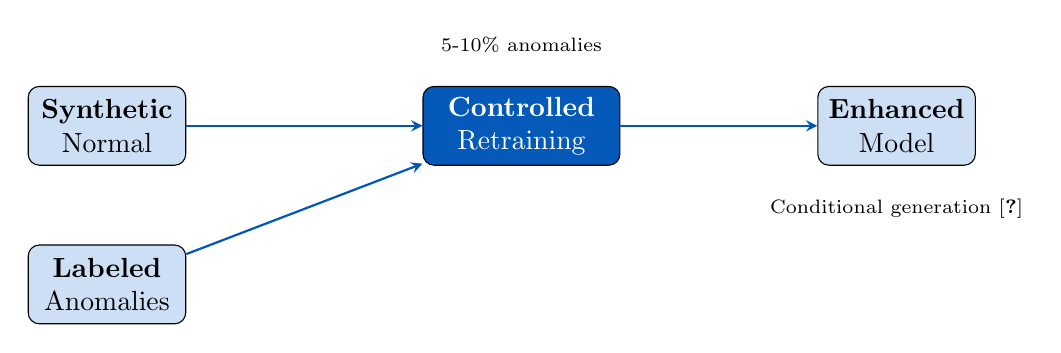
\begin{tikzpicture}[
      node distance=2.5cm,
      every node/.style={align=center},
      data/.style={draw, fill=ScienceBlue!20, rounded corners, minimum width=2cm, minimum height=1cm},
      process/.style={draw, fill=AbsoluteZero, text=white, rounded corners, minimum width=2.5cm, minimum height=1cm},
      arrow/.style={thick, VUBlue, ->, >=stealth}
    ]
      \node[data] (normal) {\textbf{Synthetic}\\Normal};
      \node[data, below=1cm of normal] (anomaly) {\textbf{Labeled}\\Anomalies};
      \node[process, right=3cm of normal] (retrain) {\textbf{Controlled}\\Retraining};
      \node[data, right=of retrain] (output) {\textbf{Enhanced}\\Model};
      \draw[arrow] (normal) -- (retrain);
      \draw[arrow] (anomaly) -- (retrain);
      \draw[arrow] (retrain) -- (output);
      % Merge indicator
      \node[above=0.3cm of retrain, font=\scriptsize] {5-10\% anomalies};
      \node[below=0.3cm of output, font=\scriptsize] {Conditional generation \cite{wangDetectingAnomalousTrajectories2018}};
    \end{tikzpicture}
  \end{center}
  \vspace{1em}
  \begin{alertblock}{Controlled Iterative Improvement}
    \small
    The model is enhanced, but requires strict controls to prevent degradation:
    \begin{itemize}
        \item \textbf{Limited Cycles:} Iterate only 3-5 times to avoid quality decay and exponential data needs \cite{seddikHowBadTraining2024}.
        \item \textbf{Monitor Stability:} Continuously watch for model collapse, where the generator forgets diversity and produces low-quality samples \cite{gerstgrasserModelCollapseInevitable2024}.
    \end{itemize}
  \end{alertblock}
\end{frame}

% --- Rule-Based Anomaly Classification ---
\begin{frame}{Rule-Based Anomaly Classification}
  % Use columns for side-by-side layout
  \begin{columns}[T,onlytextwidth]
    \begin{column}{0.42\textwidth}
      \begin{block}{Variable Definitions}
        \scriptsize
        \begin{tabular}{@{}l p{.65\linewidth}@{}}
          $AL_r$ & Length of anomalous trajectory $A_r$ \\
          $AT_r$ & Duration (time) of anomalous trajectory $A_r$ \\
          $NL_{value}$ & Avg. length of normal trajectories \\
          $NT_{value}$ & Avg. duration of normal trajectories \\
          $L_\rho$ & Length threshold (tolerance) \\
          $T_\rho$ & Time threshold (tolerance) \\
        \end{tabular}
      \end{block}
    \end{column}
    \begin{column}{0.48\textwidth}
      \begin{block}{Four Anomalous Behavior Patterns \cite{wangDetectingAnomalousTrajectories2018}}
        \scriptsize
        Given $A_r$ with $AL_r$, $AT_r$, and normal averages $NL_{value}$, $NT_{value}$:
        \begin{itemize}
          \item \textbf{Abp1}: $AL_r \leq NL_{value} + L_\rho$ and $AT_r \leq NT_{value} + T_\rho$
          \item \textbf{Abp2}: $AL_r \leq NL_{value} + L_\rho$ and $AT_r > NT_{value} + T_\rho$
          \item \textbf{Abp3}: $AL_r > NL_{value} + L_\rho$ and $AT_r \leq NT_{value} + T_\rho$
          \item \textbf{Abp4}: $AL_r > NL_{value} + L_\rho$ and $AT_r > NT_{value} + T_\rho$
        \end{itemize}
      \end{block}
    \end{column}
  \end{columns}
  
  \vspace{0.5em}
  \begin{alertblock}{Pattern Interpretation}
    \footnotesize
    \textbf{Abp1}: Efficient routes (rush hour alternatives) | \textbf{Abp2}: Traffic delays | \textbf{Abp3}: Fast detours | \textbf{Abp4}: Fraudulent behavior
  \end{alertblock}
\end{frame}

% --- Privacy Framework Part 1 ---
\begin{frame}{Privacy Framework: Generative \& Architectural Defenses}
    \begin{block}{1. Generative Privacy: Decoupling from Real Data}
        \small
        The core privacy guarantee comes from the generative nature of the DiffTraj model, which breaks the link between synthetic outputs and real inputs.
        \begin{itemize}
            \item \textbf{Generation from Noise:} Synthetic trajectories are built from random noise, not by perturbing real trajectories. This prevents direct re-identification \cite{zhuDiffTrajGeneratingGPS2023}.
            \item \textbf{Instance-Level Privacy Unit:} The model operates on entire trajectories, not individual locations, protecting against correlation attacks that exploit intra-trajectory patterns \cite{buchholzSystematisationKnowledgeTrajectory2024}.
        \end{itemize}
    \end{block}
    
    \vspace{1em}
    \begin{block}{2. Architectural Defense: Preventing Model Collapse}
        \small
        The framework's iterative process is designed to prevent privacy erosion and utility decay over time.
        \begin{itemize}
            \item \textbf{Data Accumulation:} Real data is always preserved. We only add synthetic data, never replace the original, which is a key strategy to prevent model collapse and information loss \cite{gerstgrasserModelCollapseInevitable2024}.
        \end{itemize}
    \end{block}
\end{frame}

% --- Privacy Framework Part 2 ---
\begin{frame}{Privacy Framework: Threat Mitigation}
    \begin{alertblock}{3. Practical Defense: Resisting Known Attacks}
        \small
        The framework provides resilience against two primary privacy threats for trajectory data \cite{buchholzSystematisationKnowledgeTrajectory2024}:
        \begin{itemize}
            \item \textbf{Membership Inference Attacks (MIA):} Because synthetic data is decoupled, an attacker cannot easily determine if a real trajectory was in the training set.
            \item \textbf{Attribute Inference Attacks (AIA):} The model learns general patterns, not individual-specific details, making it hard to infer sensitive attributes from the output.
        \end{itemize}
    \end{alertblock}

    \vspace{1em}
    \begin{block}{Summary: Multi-Layered Privacy}
      \centering
      \large
      This approach combines generative, architectural, and practical defenses to create a robust, privacy-by-design solution.
    \end{block}
\end{frame}

% --- Evaluation & Results ---
\begin{frame}{Evaluation Framework: Data \& Quality}
    \begin{block}{1. Datasets: Benchmarking on Real-World Scenarios}
        \small
        The framework is evaluated using standard public taxi-route datasets, which are common benchmarks for trajectory analysis and generation research \cite{zhuDiffTrajGeneratingGPS2023}.
        \begin{itemize}
            \item \textbf{Beijing Taxi Trajectories:} The primary dataset for model development and training.
            \item \textbf{Chengdu \& Xi'an:} Used for cross-city validation to test the model's generalization capabilities across different urban environments.
        \end{itemize}
    \end{block}
    
    \vspace{1em}
    
    \begin{block}{2. Quality: Statistical Fidelity}
        \small
        We use the \textbf{SDMetrics} library to assess how well the synthetic data captures the statistical properties of the real data, including univariate distributions and bivariate correlations \cite{espinosaQualitySyntheticGenerated2023}.
    \end{block}
\end{frame}

\begin{frame}{Evaluation Framework: Utility \& Privacy}
    \begin{block}{3. Utility: Detection Performance}
        \small
        The ultimate test is model utility. We measure \textbf{Precision, Recall, and F1-Score} to evaluate the anomaly detector's performance when trained on the enhanced synthetic dataset \cite{mbuyaTrajectoryAnomalyDetection2024}.
    \end{block}

    \vspace{1em}
    
    \begin{alertblock}{4. Privacy: Resilience to Attacks}
        \small
        The framework's privacy is validated by assessing its resilience against common threats, particularly \textbf{Membership Inference Attacks (MIA)}, ensuring that generated data does not leak information about the original training set \cite{buchholzSystematisationKnowledgeTrajectory2024}.
    \end{alertblock}
\end{frame}

% --- Key Contributions ---
\begin{frame}{Key Contributions}
  \begin{block}{}
    \begin{enumerate}
      \item \textbf{First integrated DiffTraj + LM-TAD framework} for privacy-preserving trajectory generation
      \item \textbf{Bootstrap methodology} that generates anomalies without pre-labeled datasets
      \item \textbf{A multi-layered privacy framework} combining generative guarantees with architectural defenses to preserve utility.
    \end{enumerate}
  \end{block}
  
  \vspace{1em}
  \begin{alertblock}{Current Status}
    \centering
    Phase 1 implementation in progress | Phases 2-3 planned for completion by thesis defense
  \end{alertblock}
\end{frame}

% --- Thank You ---
\begin{frame}[plain]
  \centering
  \Huge \textbf{Thank You}
  
  \vspace{0.5em}
  \Large \textbf{Questions \& Discussion}
  
  \vspace{2em}
  \begin{block}{}
    \centering
    \textbf{Privacy by Design} | \textbf{Generative Bootstrap} | \textbf{Data Utility}
  \end{block}
\end{frame}

% --- References ---
\begin{frame}[allowframebreaks]{References}
  \footnotesize
  \printbibliography[heading=none]
\end{frame}

\end{document} 